%%%%%%%%%%%%%%%%%%%%%%%%%%%%%%%%%%%%%%%%%
% Beamer Presentation
% LaTeX Template
% Version 1.0 (10/11/12)
%
% This template has been downloaded from:
% http://www.LaTeXTemplates.com
%
% License:
% CC BY-NC-SA 3.0 (http://creativecommons.org/licenses/by-nc-sa/3.0/)
%
%%%%%%%%%%%%%%%%%%%%%%%%%%%%%%%%%%%%%%%%%

%----------------------------------------------------------------------------------------
%	PACKAGES AND THEMES
%----------------------------------------------------------------------------------------

\documentclass{beamer}
\usepackage[natbib=true,style=authoryear,backend=bibtex,useprefix=true]{biblatex}
\usepackage[absolute,overlay]{textpos}

\PassOptionsToPackage{height=1cm}{beamerouterthemesidebar}
\mode<presentation> {

% The Beamer class comes with a number of default slide themes
% which change the colors and layouts of slides. Below this is a list
% of all the themes, uncomment each in turn to see what they look like.

%\usetheme{default}
%\usetheme{AnnArbor}
%\usetheme{Antibes}
%\usetheme{Bergen}
%\usetheme{Berkeley}
%\usetheme{Berlin}
%\usetheme{Boadilla}
%\usetheme{CambridgeUS}
%\usetheme{Copenhagen}
%\usetheme{Darmstadt}
%\usetheme{Dresden}
\usetheme{Frankfurt}
%\usetheme{Goettingen}
%\usetheme{Hannover}
%\usetheme{Ilmenau}
%\usetheme{JuanLesPins}
%\usetheme{Luebeck}
%\usetheme{Madrid}
%\usetheme{Malmoe}
%\usetheme{Marburg}
%\usetheme{Montpellier}
%\usetheme{PaloAlto}
%\usetheme{Pittsburgh}
%\usetheme{Rochester}
%\usetheme{Singapore}
%\usetheme{Szeged}
%\usetheme{Warsaw}

% As well as themes, the Beamer class has a number of color themes
% for any slide theme. Uncomment each of these in turn to see how it
% changes the colors of your current slide theme.

%\usecolortheme{albatross}
%\usecolortheme{beaver}
%\usecolortheme{beetle}
%\usecolortheme{crane}
%\usecolortheme{dolphin}
%\usecolortheme{dove}
%\usecolortheme{fly}
%\usecolortheme{lily}
%\usecolortheme{orchid}
%\usecolortheme{rose}
%\usecolortheme{seagull}
%\usecolortheme{seahorse}
\usecolortheme{whale}
%\usecolortheme{wolverine}
\usepackage{hyperref}       % hyperlinks
\usepackage{amsfonts}       % blackboard math symbols
\usepackage{nicefrac}       % compact symbols for 1/2, etc.
\usepackage{microtype}      % microtypography
%\setbeamertemplate{footline} % To remove the footer line/page numbering in all slides uncomment this line
\setbeamertemplate{footline}[page number] % To replace the footer line in all slides with a simple slide count uncomment this line

%\setbeamertemplate{navigation symbols}{} % To remove the navigation symbols from the bottom of all slides uncomment this line
}
\logo{
\includegraphics[scale=0.03]{utt}}
%\logo{\includegraphics[width=\beamer@sidebarwidth,height=\beamer@headheight]{example-image-a}}
\usepackage{graphicx} % Allows including images
\usepackage{booktabs} % Allows the use of \toprule, \midrule and \bottomrule in tables
\usepackage{subfig}
\usepackage{caption}
\usepackage{mathabx}
\usepackage{wrapfig}
\usepackage{tikz}
\usepackage{animate}
\usepackage{graphicx}
\usepackage{amssymb}
\usepackage{url}
\usepackage{algorithm}
\usepackage{algorithmicx}
\usepackage{algpseudocode}
\usepackage{caption}
%\usepackage{subcaption}
\usepackage{booktabs}
\usetikzlibrary{shapes.geometric, arrows}
\setbeamertemplate{itemize subitem}{\scriptsize$\blacktriangleright$}
%\usepackage{mathtools} % amsmath with fixes and additions
%\usepackage{amsmath}
\usepackage{url}
\usepackage{algorithm}
\usepackage{algorithmicx}
\usepackage{algpseudocode}
\usepackage{caption}
\usepackage{subcaption}
\usepackage{booktabs}
\usepackage{mathtools, xparse}
\usepackage{epstopdf}
%\usepackage{commath}
\usepackage{float}
\usepackage{multirow}
\usepackage{pdflscape}
\usepackage{adjustbox}
\usepackage{bm}
\usepackage{svg}
\usepackage{relsize}
\newcommand{\bigqm}[1][1]{\text{\larger[#1]{\textbf{?}}}}
\usepackage{amssymb,amsmath,amsthm}
\usepackage{algcompatible, amsmath}
\newcommand*{\colorboxed}{}
\def\colorboxed#1#{\colorboxedAux{#1}}
\newcommand*{\colorboxedAux}[3]{%
  % #1: optional argument for color model
  % #2: color specification
  % #3: formula
  \begingroup
    \colorlet{cb@saved}{.}%
    \color#1{#2}%
    \boxed{%
      \color{cb@saved}%
      #3%
    }%
  \endgroup
}
\setbeamercovered{invisible}
\usepackage{color, colortbl}
\usepackage[table, svgnames, dvipsnames]{xcolor}
%\usepackage{makecell, cellspace, caption}
\hypersetup{pdfpagemode=FullScreen}
\definecolor{LightCyan}{rgb}{0.88,1,1}
\definecolor{DeepCyan}{rgb}{0.60,1,1}
\addbibresource{sample.bib}
\newcommand{\comment}[1]{}
\graphicspath{{./Figures/}}
%\usepackage{subcaption}
%----------------------------------------------------------------------------------------
%	TITLE PAGE
%----------------------------------------------------------------------------------------
\title[ ]{\huge On Root Cause Analysis\\\scriptsize A case study with Supervised and Unsupervised Machine Learning} % The short title appears at the bottom of every slide, the full title is only on the title page
\author[E.I.K]{Kenneth EZUKWOKE\inst{1}, Samuel GRUFFAZ\inst{2}, Mouhamadou-Lamine NDAO\inst{3}, Amine MELAKHSOU\inst{1}\\
\scriptsize{\texttt{\{ifeanyi.ezukwoke, amine.melakhsou\}@emse.fr}}
\scriptsize{\texttt{\{samuel.gruffaz@ens-paris-saclay.fr, mlndao@cesi.fr\}}}
%\footnotesize \textcolor{blue}{\textit{Ph.D. Canon destructive inspectiondate}}:\quad Kenneth EZUKWOKE\inst{1}\\ \qquad \qquad \quad
%\textcolor{blue}{\textit{Director}}: \quad Prof. Mireille BATTON-HUBERT \inst{1} \\ \textcolor{blue}{\textit{Co-director}}: %\quad Prof. Xavier BOUCHER \inst{1}\\
%\textcolor{blue}{\textit{Co-supervisor}}: \quad Asst. Prof. Anis HOAYEK \inst{1}
}
\institute[ENSM-SE] % Your institution as it will appear on the bottom of every slide, may be shorthand to save space
{
	
\includegraphics[height=1.1cm]{emse}
\includegraphics[height=0.85cm]{ens}
\includegraphics[height=1.1cm]{cesi}\\
	\inst{1}{Mines Saint-Etienne}, \inst{2}{ENS Paris-Saclay}, \inst{3}{CESI}\and
	
\includegraphics[height=0.5cm]{gdr} 
\includegraphics[height=0.5cm]{cnrs}\\
	%\inst{2}{STMicroelectronics}
	%\textit{\{ifeanyi.ezukwoke\}@etu.univ-st-etienne.fr} % Your email address
}
\date{\today}
\begin{document}
\setlength{\abovedisplayskip}{2pt}
\setlength{\belowdisplayskip}{2pt}
\begin{frame}
\titlepage % Print the title page as the first slide
\end{frame}

%\begin{frame}{Outline}
%\scriptsize
%  \tableofcontents
%\end{frame}

%---------Introduction---------------------------------
\section{Root Cause Analysis}
\subsection{Introduction}
\begin{frame}
		\frametitle{Introduction}
		\begin{block}{Root Cause Analysis for Process Mining}
			\begin{itemize}
				\item Certain units generate a violation of BPMN (Business Process Model and Notation). It is then interesting to seek to explain the cause of this violation, which takes the form of a binary variable.
                \item Variables describing the units (supplier, delivery person, type of industrial part, etc.) were used to explain these violations, without much success.
				%\item It uses existing content like text, audio files, or images to create new plausible content. 
			\end{itemize}
		\end{block}
		\begin{exampleblock}{Research objective}
		\begin{itemize}
				\item Design and adapt a statistical learning model to predict violations and \textbf{explain} the variables causing the violations. The end goal is to have diagnotstic/exploration tools for a software.
			\end{itemize}
		\end{exampleblock}
\end{frame}

\begin{frame}
		\frametitle{Data}
		\begin{block}{Notations}
			\begin{itemize}
                \item We are looking to $N$ individuals.
				\item For any $i\in [N]$, $X_i$ is a sequence of Event with their time of size $T_i$, ex: [(E4, 0 day), (E2, 1 day),(E2, 1.5 day) ], $T_i=3$.
                \item For any $i\in [N]$, $Y_i\in \{0,1\}^m$ with $m \in \mathbb{N}^*$ (labels related to the violations).
				%\item It uses existing content like text, audio files, or images to create new plausible content. 
			\end{itemize}
		\end{block}
		\begin{exampleblock}{Formal objective}
		\begin{itemize}
				\item There are two datasets, a toy's one and a real one.
                \item  Toys dataset: $N>10^6$ and the violations are linked to subsequence of events (ex: "15-13" in "16-15-13"), $m=9$.
                \item  Real dataset: $N\approx 10^5$ and the violations are unknown, $m=5$.
			\end{itemize}
		\end{exampleblock}
\end{frame}


\begin{frame}
		\frametitle{Summary}
        From the more to the less complex methods:
		\begin{itemize}
		    \item BiLSTM-CRF on the whole sequences.
            \item Explainable One-class classification with the transition profile.
            \item Logistic Regression on the three first step of the Process.
            \item Event clustering with Levenshtein distance.
            
		\end{itemize}
  \vspace{5mm}
  BiLSTM= Bidirectionnal Long Short Term Memory\\
  CRF= Conditional Random Fields
\end{frame}
%--Resultss

\section{BiLSTM-CRF}
\subsection{Evaluation}
\begin{frame} %---EV 1
%\begin{block}{Training BiLSTM-CRF}
\begin{columns}
\begin{column}{0.5\textwidth}
\begin{block}{\scriptsize Training BiLSTM-CRF}
   \begin{itemize}
        \scriptsize
        \item Training a CRF parameterized by a BiLSTM neural network. Forward pass with Vertibi algorithm to learn transitions and backward pass by Negative Log likelihood to compute loss.
        \item Predictor sequence example ”4-7-3-6-2-8-1” with a vector
target, ”0 0 0 0 0 0”. The strings are mapped to corresponding number for
modeling.
\end{itemize}
\end{block}
\end{column}
\begin{column}{0.5\textwidth}  %%<--- here
    \begin{center}
     \begin{figure}[!h]
            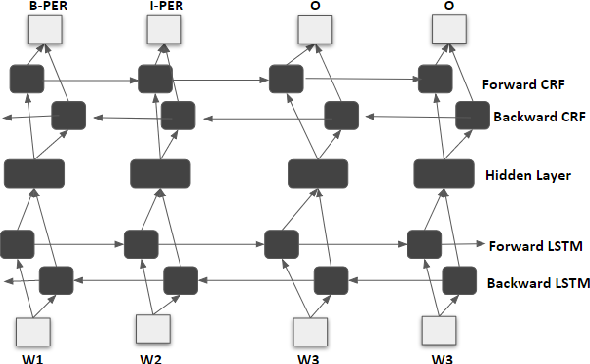
\includegraphics[scale = .27]{bilstm_crf.png}
            \centering
            \caption{\scriptsize Illustration of Three Layers of LSTM with CRF head. W1:Event1}
            \label{fig1}
    \end{figure}
    \end{center}
\end{column}
\end{columns}

\begin{table}[!h]
\begin{tabular}{cccc}
\hline
                & \multicolumn{3}{c}{Evaluation metric} \\ \hline
                & Precision    & Recall    & F1-score   \\ \hline
Toy violations  & 0.79         & 0.78      & 0.78       \\ \hline
\rowcolor[HTML]{C0C0C0} Real violations & -- {\color{red}$^{0.99}$} & -- {\color{red}$^{0.99}$} & -- {\color{red}$^{0.99}$}              \\ \hline
\end{tabular}
\caption{\scriptsize BiLSTM-CRF. Evaluation metric for Toy and Real datasets after training for 500 training steps on a subsample of the data ($1000$ data points). The $99\%$ F1-score on the Real dataset is biased towards the majority class with no violations.}
\end{table}
\end{frame}


%---------
\subsection{On BPMI Violations: Real Data}
\begin{frame} %---EV 1
\begin{block}{Process/EventID 1: 7-3-6-2-8-1}
		\begin{itemize}
                \scriptsize
				\item The order of above event ID or sequence yields the violations 0-0-0-0-0-1.
			\end{itemize}
\end{block}
\begin{figure}[!h]
            
\includegraphics[scale = .23]{n_item_one.png}
            \centering
            \caption{\scriptsize Latent representation of the process variables causing the violation. The score of $69.94$ indicates the best score in generating the sequence. The red label values on the sequence indicate the contribution individual subprocesses towards predicting the tag sequence $0-0-0-0-0-1$.}
            \label{fig1}
\end{figure}
\begin{block}{EventID 1: 7-3-6-2-8-1}
		\begin{itemize}
            \scriptsize
			\item The weights of the sentence in the above representation is parameterized by a BiLSTM neural network and rounded to one decimal place.
            \item The strong purple color is a strong indicator of a violation. Here, the model indicates event $2$, with high negative value, as a possible flag of the violation.
			\end{itemize}
\end{block}
\end{frame}

\subsection{On BPMI Violations: Toy Data}
\begin{frame} %---EV 1
\begin{block}{Process/EventID 1: 14-10-11-4-13-12-9-7-1-18-17-15-16}
		\begin{itemize}
                \scriptsize
				\item Violations for this sequence is observed for "1\_First\_appears\_as\_Seventh"
			\end{itemize}
\end{block}
\begin{figure}[!h]
            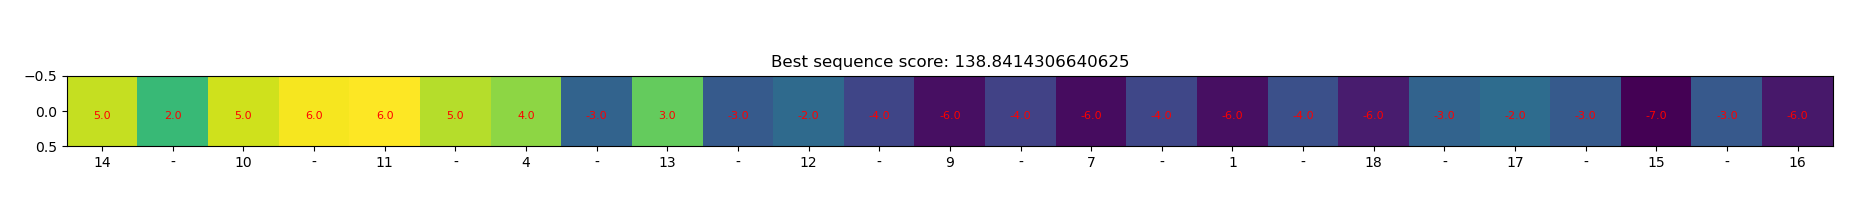
\includegraphics[scale = .23]{item_zero.png}
            \centering
            \caption{\scriptsize Latent representation of the process variables causing the violation. The score of $138.84$ indicates the best score in generating the sequence. The red label values on the the sequence indicate the contribution or emission weights of the individual subprocesses towards predicting the tag sequence $0-0-0-0-0-0-0-1-0$.}
            \label{fig1}
\end{figure}
\begin{block}{EventID 1: 14-10-11-4-13-12-9-7-1-18-17-15-16}
		\begin{itemize}
            \scriptsize
			\item The weights of the sentence in the above representation is parameterized by a BiLSTM neural network and rounded to one decimal place.
            \item The strong purple color "maybe" a strong indicator of a a violation. Sequences $9-7-1-18$ with high negative values before a violation is flagged.
			\end{itemize}
\end{block}
\begin{alertblock}{Limitation}
		\begin{itemize}
            \scriptsize
			\item Training a forward/backward pass of the CRF is time consuming.
			\end{itemize}
\end{alertblock}
\end{frame}

% One class-----------
\section{One-class classification}

\subsection{Introduction}
\begin{frame}{One-class classification for detecting and explaining violations} %---EV 1

\begin{block}{Principle}
Violations are rare in nature and  their labels are often unavailable. It is then important to develop an explainable anomaly detection model to detect and explain them.

Proposed approach:
\begin{columns}
    \begin{column}{0.7\textwidth}
        \begin{itemize}
            \item Cluster some violation-free event traces. 
            \item Flag new event traces that are so far from the closest centroid as violations
    \end{itemize}
    \end{column}
    \begin{column}{0.3\textwidth}
        \begin{figure}{\textwidth}
        \centering
        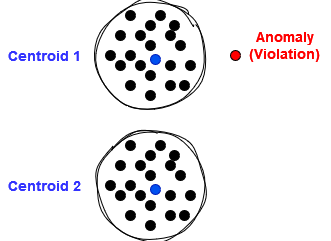
\includegraphics[scale=0.4]{ROOTCAUSE/Figures/anom_det.png}
        \label{fig:my_label}
    \end{figure}
    \end{column}
\end{columns}

\end{block}
\textbf{Issue}: Event traces are of different lengths, how to cluster them?
\end{frame}

\subsection{Transition profile}
\begin{frame} %---EV 1

\begin{block}{Transition profile}
Transition profile is an N $\times$ N matrix where N is the number of possible jobs in the process where for each cell i-j we count the number of the occurrence of the sequence (i-j) in the event trace. \\
The matrix is then flattened to form a feature vector.

\end{block}
\begin{figure}
    \centering
    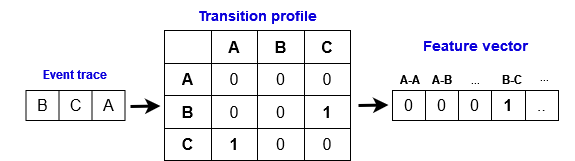
\includegraphics[scale=0.4]{ROOTCAUSE/Figures/trans_profil.png}
    \caption{Transition profile and the feature vector.}
    \label{fig:my_label}
\end{figure}

The feature vectors are of the same length and ready to use for clustering. 

\end{frame}

\subsection{Evaluation}
\begin{frame}{Evaluation} %---EV 1
\begin{block}{Training}
		\begin{itemize}
                \item Training is done by clustering the feature vectors of 100 violation-free event traces.
				\item At test time, flag new event traces as violation if the distance from the centroid is higher than a threshold.
			\end{itemize}
\end{block}
\begin{table}[!h]
\begin{tabular}{ccccc}
\hline
                & \multicolumn{3}{c}{Evaluation metric}& Prediction time \\ \hline
                & Precision    & Recall    & F1-score &  \\ \hline
Real violations data &    0.858&   0.733 &0.766    &0.02 seconds        \\ \hline
\end{tabular}
\caption{Obtained results.}
\end{table}
\end{frame}


\subsection{Explainability}
\begin{frame}{Explainability} %---EV 1
\begin{wrapfigure}{r}{0.5\textwidth}
    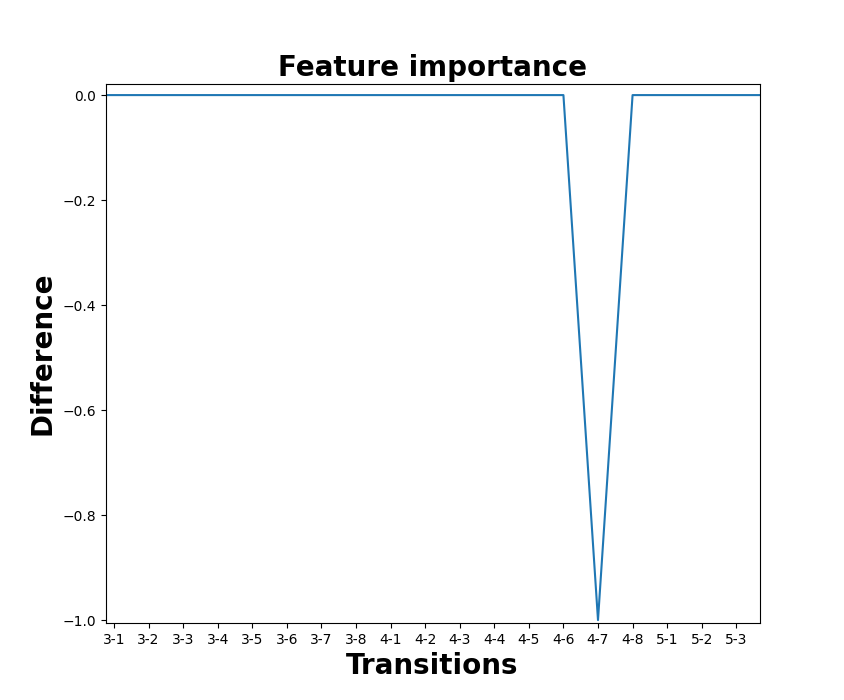
\includegraphics[scale=0.25]{ROOTCAUSE/Figures/Feature_importance.png}
\end{wrapfigure}

\begin{block}{Explainability by feature importance}
Feature importance is estimated here as the point-wise difference between the transition feature of the abnormal event and the centroid. 
\end{block}

Example: for $violation\_6$, we get -1 for the transition '4-7‘. Interpretation:  The sequence '4-7‘ is missing, which explains the violation. \\
\begin{itemize}
    \item Normal event trace: [4, 7, 3, 6, 2, 8, 1]
    \item $violation\_6$ event: [7, 3, 6, 2, 8, 1]
\end{itemize}


\end{frame}

\begin{frame}{Explainability}
Following the proposed approach, here are the explanation for each violation type: 
\textbf{Normal sequence [4-7-3-6-2-8-1]}
\begin{table}[]
    \centering
    \begin{tabular}{c|c|c}
         Violation number& Explanation & Example  \\
         \hline
         $V_1$& Normal &[4-7-3-6-2-8-1] \\
         \rowcolor[HTML]{C0C0C0}$V_2$& Normal &[4-7-3-6-2-8-1]  \\
         $V_3$& 3-6 missing & [4-6-2-8-1] \\
         \rowcolor[HTML]{C0C0C0}$V_4$& 8-2 instead of 2-8&[4-7-3-6-8-2-1] \\
         $V_5$& 6-3 instead of 3-6&[4-7-6-3-2-8-1] \\
         \rowcolor[HTML]{C0C0C0}$V_6$& 4-6 missing & [7-3-6-2-8-1] \\
         
    \end{tabular}
    \caption{Obtained explanations for the violations}
    \label{tab:my_label}
\end{table}
Violation 1 and Violation 2 are not caused by an abnormal event trace. Other features, such as the mean time between jobs, must be added to the feature vector to detect and explain these violations. 
\end{frame}

%--------------------------------------
\section{Logistic Regression}
\subsection{Evaluation}
\begin{frame} %---EV 1
\begin{block}{Setup of the Logistic Regression on the real dataset}
		$X= (X_i[:3])_{i\in [N]}$, we choose the 3 first event with their reltime as input (events are onehotencoded). $Y$ is the label will be the label of each violation.
\end{block}
\begin{table}[!h]
\begin{tabular}{cccc}
\hline
                & \multicolumn{1}{c}{Evaluation metric} \\ \hline
                 & F1-score   \\ \hline
Y1  & 0.75            \\ \hline
\rowcolor[HTML]{C0C0C0}Y2&      0.99           \\ \hline
Y3&          0.99       \\ \hline
\rowcolor[HTML]{C0C0C0}Y4&        0.03         \\ \hline
Y5&        0.99         \\ \hline
\end{tabular}
\caption{F1 score of the Logistic Regression for the different violations. Remark that Y1 without time have F1 score of 0.2}
\end{table}
\end{frame}


%---------


\begin{frame} %---EV 1

\begin{figure}[!h]
            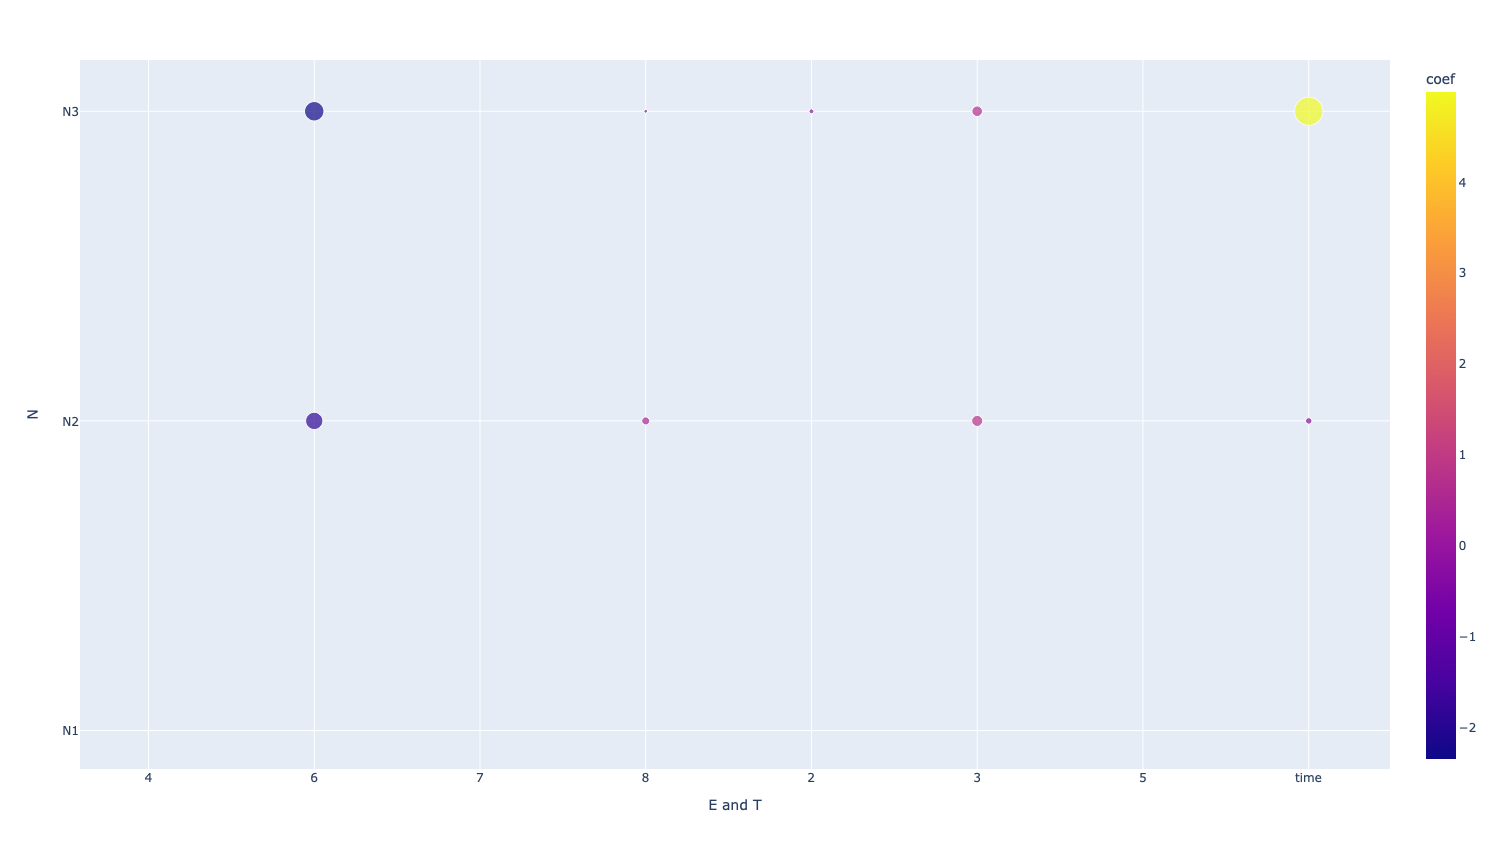
\includegraphics[scale = 0.2]{ROOTCAUSE/Figures/coefLR_Y1.png}
            \centering
            \caption{\scriptsize We choose a L1 penalty to keep only relevant coefficients. The points are bigger according to the norm of the coefficients. The points are dark when their related variables decrease the probability of having $Y=1$, the logic is reverse for light points. }
            \label{fig1dd}
\end{figure}

\end{frame}


\section{Clustering}
\subsection{Evaluation}
\begin{frame} %---EV 1
\begin{block}{Clustering sequential data}
\begin{itemize}
%\scriptsize 
\item The objective is to use a non-supervised approach to identify clusters of events that contain violations.
\end{itemize}
\end{block}

\begin{block}{Methodology}
\begin{itemize}
%\scriptsize 
\item \textbf{$K$-mode} (\cite{mastrogiannis2009cl}): an approach used to group categorical datasets into homogeneous clusters.
\item With similarity measured by the \textbf{Levenshtein distance}(\cite{yujian2007normalized}).
\item Comparison between the partition obtained by k-mode and the types of violations observed by an \textbf{adjusted rand index} (\cite{steinley2004properties}).
\end{itemize}
\end{block}
\end{frame}

\begin{frame}{Results}

\begin{minipage}[t]{0.5\linewidth}
\begin{figure}[ht]
        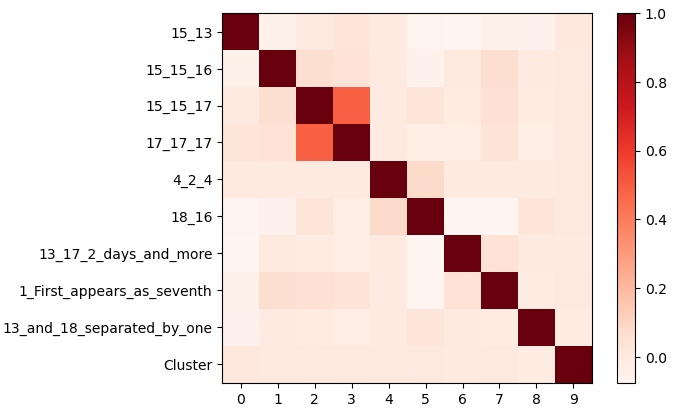
\includegraphics[width=1\textwidth,scale=0.3]{ROOTCAUSE/Figures/experiment_data.png}
        \caption{Similarity between clusters with simulation data.}
        \label{fig:my_label}
\end{figure}
\end{minipage}\hfill
\begin{minipage}[t]{0.5\linewidth}
\begin{figure}[ht]
        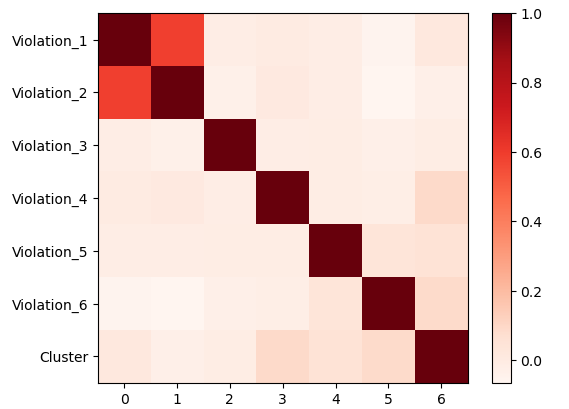
\includegraphics[width=.9\textwidth,scale=0.2]{ROOTCAUSE/Figures/real_data.png}
        \caption{Similarity between clusters with real data.}
        \label{fig:my_label}
\end{figure}
\vspace{-0.5cm}
\begin{itemize}
   % \item 
\end{itemize}

\end{minipage}

\end{frame}


%---------

\section{Conlusion}
\begin{frame}{Conclusion}
    \begin{block}{Conclusion}
    \begin{itemize}
        \item There are severals methods to tackle the problem and we should select it according to what we are looking for and the kind of violation.
        \item It seems that there are signals both in the ordering of events and their relative times, but expert knowledge are needed to draw robust conclusions.
    \end{itemize}
    \end{block}
\end{frame}



%last slide

\subsection*{Thank you}
\begin{frame}{Thank you}
    \begin{block}{Thank you}
    Thank you for your attention...
    \end{block}
\end{frame}

\appendix


\begin{frame} %EV -2
\begin{block}{Process/EventID 2: 14-10-9-12-17-15-15-13-16}
		\begin{itemize}
                \scriptsize
				\item Violations for this sequence is observed for "15\_15\_17" and "1\_First\_appears\_as\_Seventh"
			\end{itemize}
\end{block}
\begin{figure}[!h]
            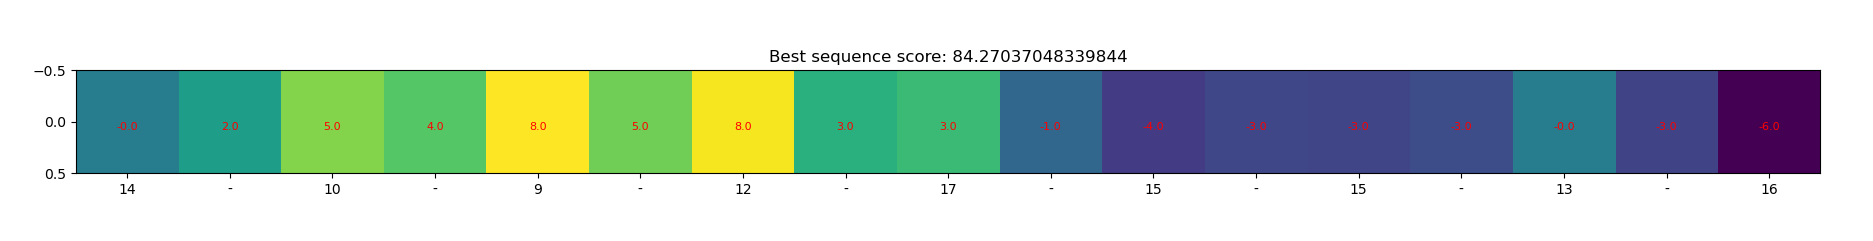
\includegraphics[scale = .23]{item_two.png}
            \centering
            \caption{\scriptsize Latent representation of the process variables causing the violation.  The red label values on the sequence indicate the contribution or emission weights of the individual subprocesses towards predicting the tag sequence $0-1-0-0-0-0-0-1-0$.}
            \label{fig2}
\end{figure}
\begin{block}{EventID 2: 14-10-9-12-17-15-15-13-16}
		\begin{itemize}
            \scriptsize
			\item The weights on the representation indicates a violation from subsequence "15-15" but especially on the first "15".
			\end{itemize}
\end{block}
\end{frame}


\begin{frame} %EV -3
\begin{block}{Process/EventID 3: 14-10-9-12-17-15-15-13-16}
		\begin{itemize}
                \scriptsize
				\item Violations for this sequence is observed for "15\_13"
			\end{itemize}
\end{block}
\begin{figure}[!h]
            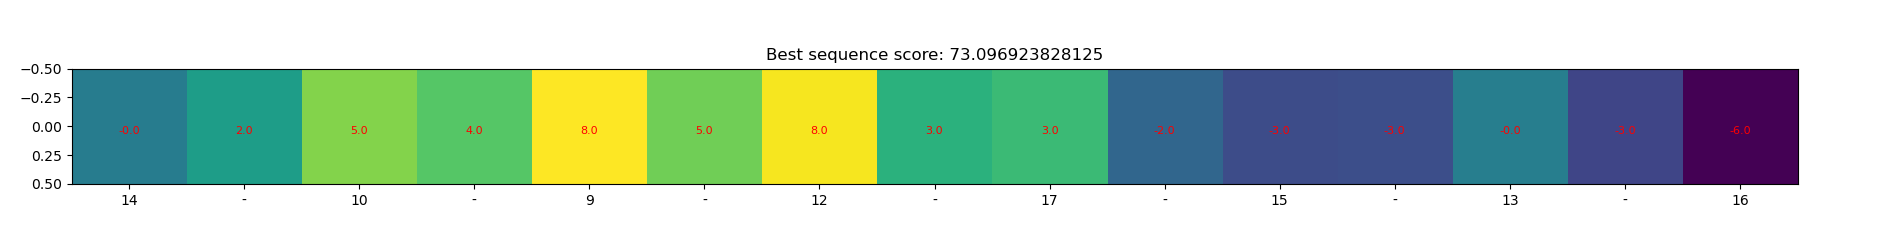
\includegraphics[scale = .23]{item_three.png}
            \centering
            \caption{\scriptsize Latent representation of the process variables causing the violation.  The red label values on the the sequence indicate the contribution or emission weights of the individual subprocesses towards predicting the tag sequence $1-0-0-0-0-0-0-0-0$.}
            \label{fig3}
\end{figure}
\begin{block}{EventID 3: 14-10-9-12-17-15-15-13-16}
		\begin{itemize}
            \scriptsize
			\item The weights on the representation does not visibly indicate a violation before "15\_13".
            \item Since, no early signal is observed for this violation, we can imagine the violation is caused by an unknown or hidden variable. 
			\end{itemize}
\end{block}
\end{frame}


\begin{frame} %EV -4
\begin{block}{Process/EventID 4: 14-10-11-4-13-12-9-7-1-18-17-15-16}
		\begin{itemize}
                \scriptsize
				\item Violations for this sequence is observed for "1\_First\_appears\_as\_Seventh"
			\end{itemize}
\end{block}
\begin{figure}[!h]
            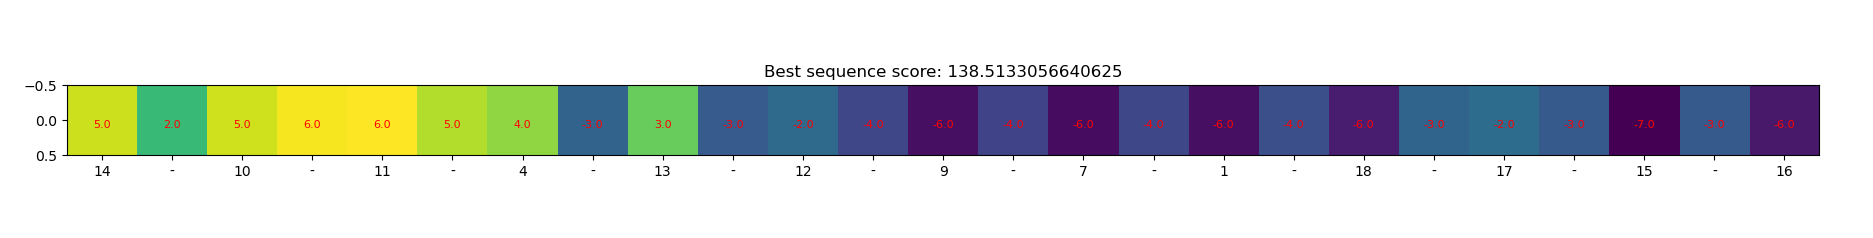
\includegraphics[scale = .23]{item_four.png}
            \centering
            \caption{\scriptsize Latent representation of the process variables causing the violation.  The red label values on the the sequence indicate the contribution or emission weights of the individual subprocesses towards predicting the tag sequence $0-0-0-0-0-0-0-1-0$.}
            \label{fig4}
\end{figure}
\begin{block}{EventID 4: 14-10-11-4-13-12-9-7-1-18-17-15-16}
		\begin{itemize}
            \scriptsize
			\item The weights on the representation strongly indicate a violation for the subsequence 9-7-1-18. We observe an early signal before the violation is flagged.
			\end{itemize}
\end{block}
\end{frame}


\begin{frame} %EV -6
\begin{block}{Process/EventID 5: 14-10-11-13-12-9-17-15-15-16}
		\begin{itemize}
                \scriptsize
				\item Violations for this sequence is observed for "15\_15\_16"
			\end{itemize}
\end{block}
\begin{figure}[!h]
            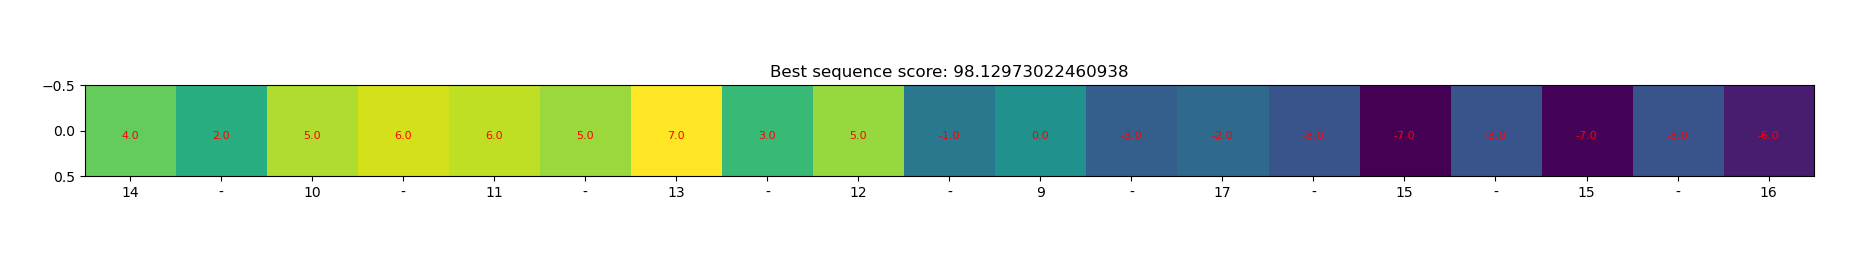
\includegraphics[scale = .23]{item_six.png}
            \centering
            \caption{\scriptsize Latent representation of the process variables causing the violation.  The red label values on the the sequence indicate the contribution or emission weights of the individual subprocesses towards predicting the tag sequence $0-1-0-0-0-0-0-0-0$.}
            \label{fig4}
\end{figure}
\begin{block}{EventID 5: 14-10-11-13-12-9-17-15-15-16}
		\begin{itemize}
            \scriptsize
			\item The weights indicated in the representation does not signal an early anomaly in the subsequences until "15\_15".
			\end{itemize}
\end{block}
\end{frame}

\begin{frame} %EV -6
\begin{block}{Process/EventID 6: 14-10-11-12-9-17-15-13-16}
		\begin{itemize}
                \scriptsize
				\item Violations for this sequence is observed for "15\_13"
			\end{itemize}
\end{block}
\begin{figure}[!h]
            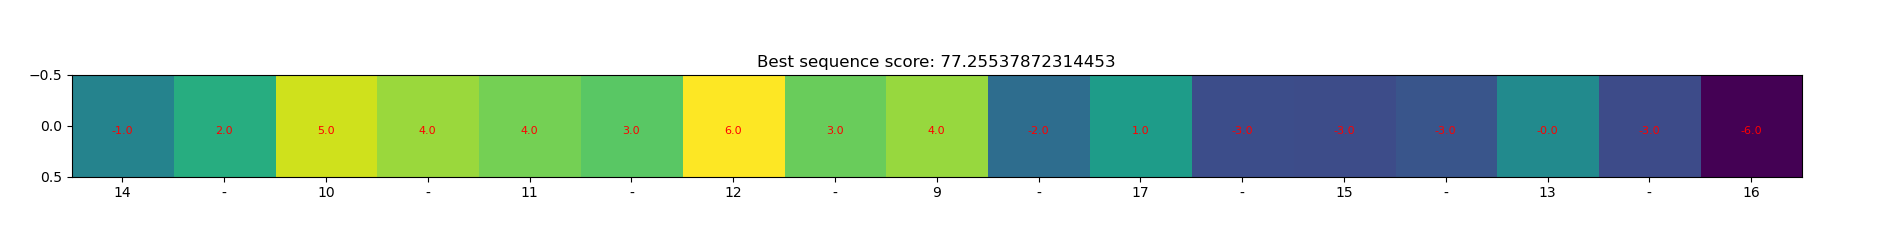
\includegraphics[scale = .23]{item_seven.png}
            \centering
            \caption{\scriptsize Latent representation of the process variables causing the violation.  The red label values on the the sequence indicate the contribution or emission weights of the individual subprocesses towards predicting the tag sequence $1-0-0-0-0-0-0-0-0$.}
            \label{fig4}
\end{figure}
\begin{block}{EventID 6: 14-10-11-12-9-17-15-13-16}
		\begin{itemize}
            \scriptsize
			\item The weights indicated in the representation does not signal an early anomaly in the subsequences until "15\_13". 
            \item However, subsequence "17" is correlated with "13" going by the weights, perhaps it is an anomaly subsequence.
			\end{itemize}
\end{block}
\end{frame}


%--- How to


\setlength{\abovedisplayskip}{8pt}
\setlength{\belowdisplayskip}{8pt}

%-----------------------------    Qualitative evaluation on FA datasets -----------------------------

%\subsection*{References}
%\begin{frame}[t, allowframebreaks]{References}
%\def\newblock{}
%\scriptsize
%\printbibliography % Use the example bibliography file sample.bib
%\end{frame}
\end{document}
%---------------------------------------------------------------------------
